\documentclass[12pt]{extarticle}
%Some packages I commonly use.
\usepackage[portuguese]{babel}
\usepackage{graphicx}
\usepackage{framed}
\usepackage[normalem]{ulem}
\usepackage{amsmath}
\usepackage{amsthm}
\usepackage{amssymb}
\usepackage{amsfonts}
\usepackage{enumerate}
\usepackage[utf8]{inputenc}
\usepackage{float}
\usepackage{gensymb}
\usepackage[top=1 in,bottom=1in, left=1 in, right=1 in]{geometry}
\usepackage{multirow}
\usepackage{caption}
\usepackage{subcaption}
\usepackage[utf8]{inputenc}
\usepackage{tikz}


%A bunch of definitions that make my life easier
\newcommand{\matlab}{{\sc Matlab} }
\newcommand{\cvec}[1]{{\mathbf #1}}
\newcommand{\rvec}[1]{\vec{\mathbf #1}}
\newcommand{\ihat}{\hat{\textbf{\i}}}
\newcommand{\jhat}{\hat{\textbf{\j}}}
\newcommand{\khat}{\hat{\textbf{k}}}
\newcommand{\minor}{{\rm minor}}
\newcommand{\trace}{{\rm trace}}
\newcommand{\spn}{{\rm Span}}
\newcommand{\rem}{{\rm rem}}
\newcommand{\ran}{{\rm range}}
\newcommand{\range}{{\rm range}}
\newcommand{\mdiv}{{\rm div}}
\newcommand{\proj}{{\rm proj}}
\newcommand{\R}{\mathbb{R}}
\newcommand{\N}{\mathbb{N}}
\newcommand{\Q}{\mathbb{Q}}
\newcommand{\Z}{\mathbb{Z}}
\newcommand{\<}{\langle}
\renewcommand{\>}{\rangle}
\renewcommand{\emptyset}{\varnothing}
\newcommand{\attn}[1]{\textbf{#1}}
\theoremstyle{definition}
\newtheorem{theorem}{Theorem}
\newtheorem{corollary}{Corollary}
\newtheorem*{definition}{Definition}
\newtheorem*{example}{Example}
\newtheorem*{note}{Note}
\newtheorem{exercise}{Exercise}
\newcommand{\bproof}{\bigskip {\bf Proof. }}
\newcommand{\eproof}{\hfill\qedsymbol}
\newcommand{\Disp}{\displaystyle}
\newcommand{\qe}{\hfill\(\bigtriangledown\)}
\setlength{\columnseprule}{1 pt}
\usepackage[utf8]{inputenc}

\usetikzlibrary{arrows,shapes,positioning}
\usetikzlibrary{decorations.markings}
\tikzstyle arrowstyle=[scale=1]
\tikzstyle directed=[postaction={decorate,decoration={markings,
    mark=at position .65 with {\arrow[arrowstyle]{stealth}}}}]
\tikzstyle reverse directed=[postaction={decorate,decoration={markings,
    mark=at position .65 with {\arrowreversed[arrowstyle]{stealth};}}}]

\title{Aula 18 - Refração e Lentes}
\author{Felipe Salvador}
\date{Atualizado em \today}

\begin{document}

\maketitle

\section{Introdução}

O segundo fenômeno ótico, que veremos nesta aula, é a \textbf{refração}. Esse fenômeno está relacionado a troca de meio de propagação da luz e como isso afeta o caminho que os raios de luz tomam. A mudança de meio em que a luz se propaga altera a velocidade que a luz se propaga.
\section{Índice de Refração ($n$)}
A quantidade que caracteriza um meio em que a luz se propaga é chamada \textbf{índice de refração} e é definida como:
\begin{equation}
    n = \frac{c}{v}
\end{equation}
\noindent em que 'c' é a velocidade da luz no vácuo ($c=3.10^8\,m/s$) e 'v' é a velocidade da luz no meio em que ela se propaga.

\textbf{Uma questão importante é que a velocidade da luz é a maior possível somente no vácuo, ou seja, $v\leq c$}. Isso faz com que o índice de refração seja: $n\geq 1$, em que $n=1$ é somente para o caso em que a luz esteja se propagando no vácuo: $v=c$.

Em termos gerais, o índice de refração é uma quantidade que me diz o quão lento a luz se propaga naquele meio em comparação com a propagação no vácuo (meio que a luz anda mais rápido). Se o indíce de refração for 'grande' (ex: n=2 ou n=2,5), isso significa que a luz está andando, naquele meio, 2 ou 2,5 vezes mais lenta que ela andaria no vácuo. 

\section{Refração}
Como já vimos, refração é o fenômeno da luz quando ela muda de meio de propagação, ou seja, quando o índice de refração (n) em que a luz está muda. Temos uma relação que descreve como a refração ocorre quando passa de um meio para o outro: \textbf{Lei de Snell}:

\begin{equation}
    n_1\,sen\,\theta_1 = n_2\,sen\,\theta_2
\end{equation}

\noindent em que $n_1,\,n_2$ são os índices de refração dos meios envolvidos e $sen\,\theta_1, sen\,\theta_2$ são os ângulos entre o raio de luz incidente/refratado e a reta normal (reta que faz um ângulo de 90$^\circ$ com a superfície que separa os meios.) Nós iremos chamar essa configuração de 2 meios com índices de refração diferentes de \textbf{dióptro plano}.

Essa equação descreve como a luz se comportará quando passar por uma troca de meio. Mas para isso, vamos analisar os 2 casos que podem acontecer. 

O primeiro caso é quando $n_2>n_1$, ou seja, a luz tá entrando um meio mais refringente (em que a luz anda mais lentamente do que quando ela andava no meio anterior).
\subsection{Caso 1 - Luz entrando num meio mais refringente ($n_2 >n_1$)}

Nesse caso, a luz tá entrando num meio em que ela anda mais lentamente do que estava. Olhando para a Lei de Snell:
\begin{equation}
    n_1\,sen\,\theta_1 = n_2\,sen\,\theta_2 \implies \frac{n_1}{n_2} = \frac{sen\,\theta_2}{sen\,\theta_1}
\end{equation}
Como $n_2>n_1$, então $\frac{n_1}{n_2} <1$. Portanto, $\frac{sen\,\theta_2}{sen\,\theta_1} <1$ também. Enfim:
\begin{equation}
    \frac{sen\,\theta_2}{sen\,\theta_1} <1 \implies \boxed{sen\,\theta_2 < sen\,\theta_1}
\end{equation}
Como o seno é expressão que cresce conforme o ângulo cresce, \textbf{isso implica que a luz quando troca de meio ela se aproxima da reta normal.} Abaixo, está um esquema para ilustrar o que acontece com a luz quando ela muda para um meio mais refringente.

\begin{figure}[H]
    \centering
    \begin{tikzpicture}

    % define coordinates
    \coordinate (O) at (0,0) ;
    \coordinate (A) at (0,4) ;
    \coordinate (B) at (0,-4) ;
    
    % media
    \fill[blue!25!,opacity=.3] (-4,0) rectangle (4,4);
    \fill[blue!60!,opacity=.3] (-4,0) rectangle (4,-4);
    \node[right] at (2,2) {$n_1$};
    \node[left] at (-2,-2) {$n_2$};

    % axis
    \draw[dash pattern=on5pt off3pt] (A) -- (B) ;

    % rays
    \draw[red,ultra thick,reverse directed] (O) -- (130:5.2);
    \draw[blue,directed,ultra thick] (O) -- (-70:4.24);

    % angles
    \draw (0,1) arc (90:130:1);
    \draw (0,-1.4) arc (270:290:1.4) ;
    \node[] at (280:1.8)  {$\theta_{2}$};
    \node[] at (110:1.4)  {$\theta_{1}$};
\end{tikzpicture}
    \caption{Esquema do processo de troca de meio de propagação da luz para o caso de $n_2>n_1$}
    \label{fig:refracao_1}
\end{figure}

\subsection{Caso 2 - Luz entrando num meio menos refringente ($n_2<n_1$)}

Nesse caso, a luz está entrando num meio em que ela anda mais rapidamente do que ela andava no meio anterior. Analisando a Lei de Snell, novamente:
\begin{equation}
     n_1\,sen\,\theta_1 = n_2\,sen\,\theta_2 \implies \frac{n_1}{n_2} = \frac{sen\,\theta_2}{sen\,\theta_1}
\end{equation}
Agora, como $n_2<n_1$, então: $\frac{n_1}{n_2} >1$. Logo: $\frac{sen\,\theta_2}{sen\,\theta_1}>1$ também. Portanto:
\begin{equation}
    \frac{sen\,\theta_2}{sen\,\theta_1}>1 \implies \boxed{sen\,\theta_2 > sen\,\theta_1}
\end{equation}
Como o seno é uma função que cresce conforme o ângulo cresce, \textbf{então isso implica que a luz quando troca de meio ela se afasta da reta normal}. Abaixo está um esquema para ilustrar o que acontece quando a luz entra um meio menos refringente:
\begin{figure}[H]
    \centering
    \begin{tikzpicture}

    % define coordinates
    \coordinate (O) at (0,0) ;
    \coordinate (A) at (0,4) ;
    \coordinate (B) at (0,-4) ;
    
    % media
    \fill[blue!25!,opacity=.3] (-4,0) rectangle (4,4);
    \fill[blue!60!,opacity=.3] (-4,0) rectangle (4,-4);
    \node[right] at (2,2) {$n_1$};
    \node[left] at (-2,-2) {$n_2$};

    % axis
    \draw[dash pattern=on5pt off3pt] (A) -- (B) ;

    % rays
    \draw[red,ultra thick,reverse directed] (O) -- (120:5.2);
    \draw[blue,directed,ultra thick] (O) -- (-40:4.24);

    % angles
    \draw (0,1) arc (90:130:0.7);
    \draw (0,-1) arc (270:300:1.9) ;
    \node[] at (295:1.4)  {$\theta_{2}$};
    \node[] at (105:1.4)  {$\theta_{1}$};
\end{tikzpicture}
    \caption{Esquema da refração da troca do meio de propagação da luz para o caso em que $n_2<n_1$}
    \label{fig:refracao_2}
\end{figure}

\subsubsection{Caso Especial - Ângulo limite ($\theta_{max}$)}

Perceba que se continuarmos a aumentar o ângulo de incidência da luz, para esse caso de refração ($n_2<n_1$), o ângulo de refração vai ficando cada vez maior. Porém, tem um momento a luz refratada sai na direção da superfície que separa os dois meios. 

Se aumentarmos um pouco mais esse ângulo de entrada agora, a luz refratada, estaria voltando para o meio em que ela estava, logo não seria mais refração.

Por isso, o caso especial é o caso em que a luz refratada sai com na direção da superfície que separa os 2 meios, ou seja, \textbf{o ângulo em que a luz refratada faz com a normal será de 90$^\circ$.} Com isso, chamamos o ângulo de incidência, que faz o ângulo de refração ser de $90^\circ$, de \textbf{ângulo limite} ($\theta_{max}$). O esquema da refração está abaixo:
\begin{figure}[H]
    \centering
    \begin{tikzpicture}

    % define coordinates
    \coordinate (O) at (0,0) ;
    \coordinate (A) at (0,4) ;
    \coordinate (B) at (0,-4) ;
    
    % media
    \fill[blue!25!,opacity=.3] (-4,0) rectangle (4,4);
    \fill[blue!60!,opacity=.3] (-4,0) rectangle (4,-4);
    \node[right] at (2,2) {$n_1$};
    \node[left] at (-2,-2) {$n_2$};

    % axis
    \draw[dash pattern=on5pt off3pt] (A) -- (B) ;

    % rays
    \draw[red,ultra thick,reverse directed] (O) -- (140:5.2);
    \draw[blue,directed,ultra thick] (O) -- (0:4);

    % angles
    \draw (0,1) arc (90:140:1);
    \draw (0,-0.5) -- (0.5,-0.5) --(0.5,0);
    \draw (0.25,-0.25) circle (1pt);
    \node[] at (110:1.4)  {$\theta_{max}$};
\end{tikzpicture}
    \caption{Esquema do caso da refração do ângulo limite}
    \label{fig:refracao_limite}
\end{figure}

Pela Lei de Snell:
\begin{equation}
    n_1\,sen\,\theta_{max} = n_2\,\underbrace{ sen\,90^\circ}_{=1} \implies \boxed{sen\,\theta_{max} = \frac{n_2}{n_1}}
\end{equation}

Isso significa que, para o caso $n_2 <n_1$, o seno do ângulo limite de incidência para que haja refração é a relação: $\frac{n_2}{n_1}$.

O que acontece se o ângulo de incidência $\theta_1 > \theta_{max}$? \textbf{A luz irá sofrer reflexão na superfície que separa os 2 meios e o outro meio funcionará como espelho.} Esse é o princípio de uma fibra ótica:

\begin{figure}[H]
    \centering
    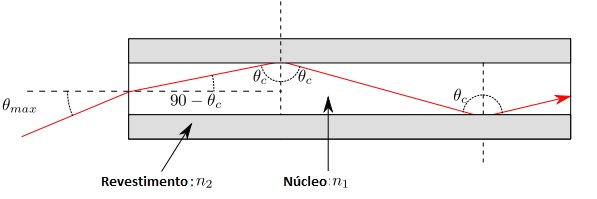
\includegraphics[width=0.8\textwidth]{fibra_otica.jpg}
    \caption{Esquema ótico do caminho que a luz faz dentro de um cabo de fibra ótica. A fibra é composta de 2 materiais: o núcleo, que possui um índice de refração $n_2$, e o revestimento, que possui um índice de refração $n_1$, de forma que $n_2<n_1$.}
    \label{fig:fibra_otica}
\end{figure}

\section{Dióptros Planos, Prismas e as Cores do arco-íris}
Nessa parte, nós iremos estudar a luz desvia quando troca de, veremos os prismas de refração e como a decomposição da luz branca nas cores do arco-íris acontece.

\subsection{Dióptros Planos}
Nessa parte, discutiremos a parte de como ver um peixe, que está dentro d'água, pode te enganar. Isso acontece porque a refração da luz dá a impressão de que o objeto imerso no outro meio esteja numa certa altura/posição em que, na realidade não está. Veja o exemplo a seguir para entender essa questão:
\begin{figure}[H]
    \centering
    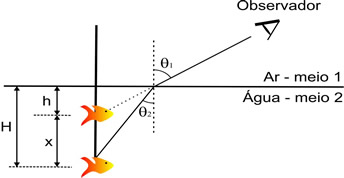
\includegraphics[width=0.6\textwidth]{dioptro2.jpg}
    \caption{Exemplo de como a refração pode enganar. O peixe aparenta estar mais perto da superfície do que realmente está.}
    \label{fig:dioptro}
\end{figure}

Para saber a real altura de onde o peixe está, nesse exemplo, pela geometria do problema e pela Lei de Snell, conseguimos derivar a seguinte expressão:
\begin{equation}
    H = \frac{n_2}{n_1}\,h
\end{equation}
\noindent em que 'H' é a altura/profundidade onde o peixe realmente está, $n_2$ é o índice de refração do meio em que o peixe está,  $n_1$ é o índice de refração do meio em que o observador está e 'h' é a altura da imagem do peixe que o observador vê.

\subsection{Prismas e as Cores do arco-íris}
O prisma é um objeto ótico que tem uma forma triangular e foi usado no começo dos estudos de ótica para demonstrar a decomposição da luz branca nas 7 cores do arco-íris.
\begin{figure}[H]
    \centering
    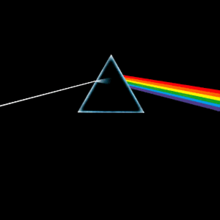
\includegraphics[width=0.4\textwidth]{Dark_Side_of_the_Moon.png}
    \caption{Capa do album mais famoso do Pink Floyd - Dark Side of the Moon. Ai a luz branca incidindo no prisma e as cores do arco-íris sendo decomposta.}
    \label{fig:pink_floyd}
\end{figure}

A questão mais importante para esse efeito acontecer é a seguinte: \textbf{para cada luz que compõe a luz branca, o índice de refração do prisma é diferente.} Em especial, a ordem dos índices de refração do prisma é:
\begin{equation}
    n_{vermelho} < n_{laranja} < n_{amarelo} < n_{verde} < n_{azul} < n_{anil} < n_{violeta}
\end{equation}

Isso é perceptível por causa do desvio que cada cor sofre. Dessa forma,as cores perto do vermelho sofrem bem menos refração do que as cores mais próximas do violeta e assim se decompõe as cores do arco-íris.

Em linhas gerais, \textbf{cores mais próximas do violeta sofrem mais desvio, por causa do prisma, do que cores mais próximas do vermelho.}

\section{Lentes}
Nessa parte, iremos estudar o principal objeto que usa a refração como o mecanismo: as lentes óticas.

As lentes são objetos que causam desvios da luz para alguma utlidade: focar os raios de luz num ponto (tipo um laser), ajustar a visão das pessoas (miopia, hipermetropia, astigmatismo).

Os nossos estudos serão somente sobre as lentes delgadas gaussianas, ou seja, as lentes são bem finas e os raios de luz passam bem próximo do centro da lente.

Ao todo, estudaremos 2 tipos de lentes:
\begin{itemize}
    \item \textbf{Lentes Convergentes} - são lentes as quais fazem que os raios de luz se aproximarem entre si e eles se cruzam sobre o foco.
    \item \textbf{Lentes Divergentes} - são lentes as quais fazem que os raios de luz se afastem entre si de forma que aparentam terem saídos de um ponto, que é o foco da lente.
\end{itemize}
\begin{figure}[H]
    \centering
    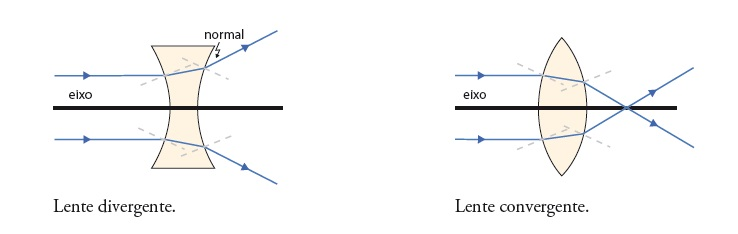
\includegraphics[width=0.9\textwidth]{lentes.jpg}
    \caption{Esquema das lentes convergentes e divergentes}
    \label{fig:lentes}
\end{figure}

Em geral, as lentes são representadas da seguinte forma:
\begin{figure}[H]
    \centering
    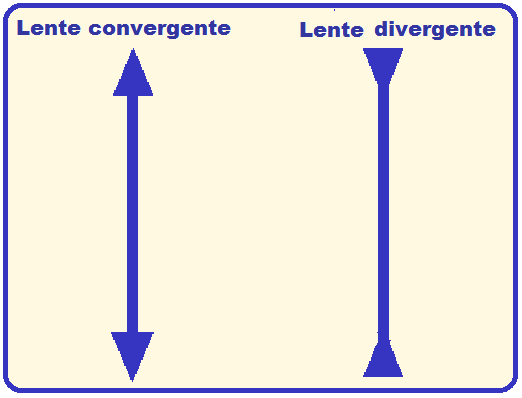
\includegraphics[width=0.4\textwidth]{representacao.png}
    \caption{Representação esquemática das lentes}
    \label{fig:lentes_representacao}
\end{figure}

Assim como nos espelhos, as lentes tem seus pontos principais:
\begin{figure}[H]
    \centering
    \begin{subfigure}[b]{0.45\textwidth}
         \centering
         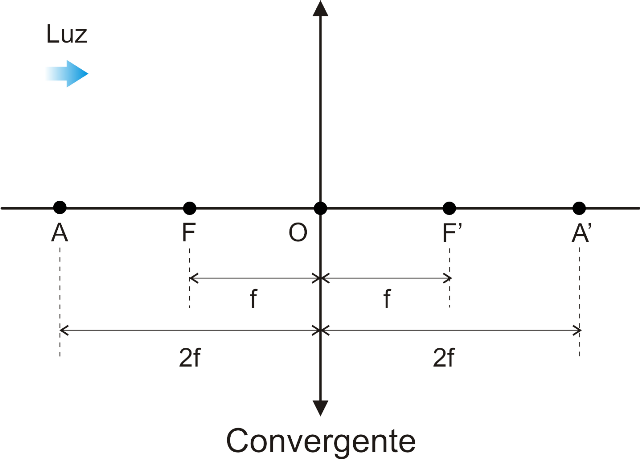
\includegraphics[width=\textwidth]{conv11.png}
         \caption{Pontos principais da lente convergente}
         \label{fig:pontos_conv}
     \end{subfigure}
     \hfill
     \begin{subfigure}[b]{0.45\textwidth}
         \centering
         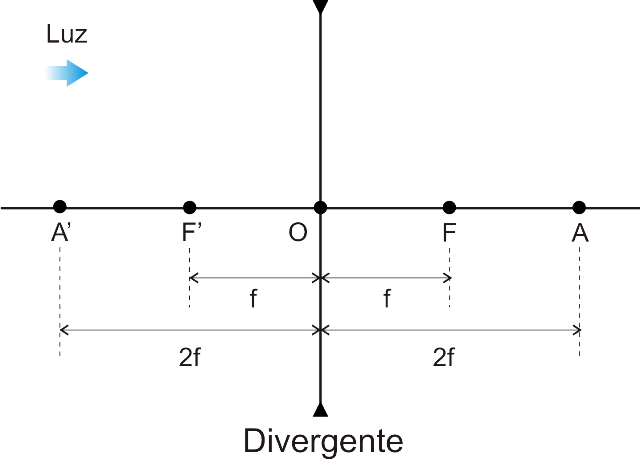
\includegraphics[width=\textwidth]{div11.png}
         \caption{Pontos principais da lente divergente}
         \label{fig:pontos_div}
     \end{subfigure}
    \caption{Pontos principais da lente: 'A' é o ponto antiprincipal, 'F' é o ponto focal e 'O' é o centro da lente. Os "A,F" são os pontos antiprincipais e foco do objeto, enquanto os "\textit{A',F'}" são os pontos antiprincipais e foco da \textbf{imagem}}
    \label{fig:pontos principais}
\end{figure}

\subsection{Raios Principais}
Assim como nos espelhos, as lentes também tem os seus raios principais, os raios mais importantes numa análise de lentes.
\begin{enumerate}
    \item \textbf{Vem paralelo e passa pelo foco}
    \begin{figure}[H]
        \centering
        \begin{subfigure}[b]{0.45\textwidth}
         \centering
         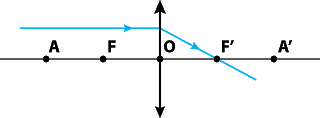
\includegraphics[width=\textwidth]{notaveis_conv_1.png}
         \caption{Lente Convergente}
         \label{fig:raios_conv_1}
     \end{subfigure}
     \hfill
     \begin{subfigure}[b]{0.45\textwidth}
         \centering
         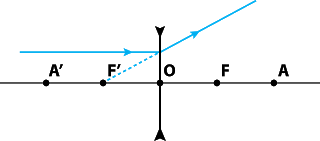
\includegraphics[width=\textwidth]{notaveis_div_1.png}
         \caption{Lente Divergente}
         \label{fig:raios_div_1}
     \end{subfigure}
    \end{figure}
    
    \item \textbf{Vem pelo foco e sai paralelo}
    \begin{figure}[H]
        \centering
        \begin{subfigure}[b]{0.45\textwidth}
         \centering
         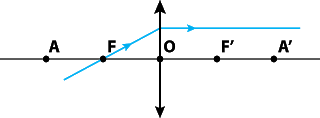
\includegraphics[width=\textwidth]{notaveis_conv_2.png}
         \caption{Lente Convergente}
         \label{fig:raios_conv_2}
     \end{subfigure}
     \hfill
     \begin{subfigure}[b]{0.45\textwidth}
         \centering
         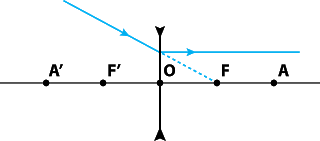
\includegraphics[width=\textwidth]{notaveis_div_2.png}
         \caption{Lente Divergente}
         \label{fig:raios_div_2}
     \end{subfigure}
    \end{figure}
    
    \item \textbf{Passa pelo Centro sem ser desviado}
    \begin{figure}[H]
        \centering
        \begin{subfigure}[b]{0.45\textwidth}
         \centering
         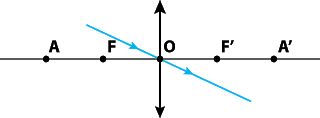
\includegraphics[width=\textwidth]{notaveis_conv_3.png}
         \caption{Lente Convergente}
         \label{fig:raios_conv_3}
     \end{subfigure}
     \hfill
     \begin{subfigure}[b]{0.45\textwidth}
         \centering
         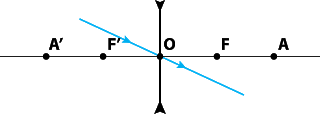
\includegraphics[width=\textwidth]{notaveis_div_3.png}
         \caption{Lente Divergente}
         \label{fig:raios_div_3}
     \end{subfigure}
    \end{figure}
    
    \item \textbf{Passa pelo Antiprincipal e sai pelo outro Antiprincipal}
    \begin{figure}[H]
        \centering
        \begin{subfigure}[b]{0.45\textwidth}
         \centering
         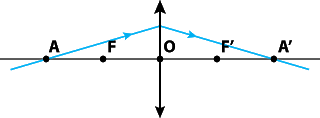
\includegraphics[width=\textwidth]{notaveis_conv_4.png}
         \caption{Lente Convergente}
         \label{fig:raios_conv_4}
     \end{subfigure}
     \hfill
     \begin{subfigure}[b]{0.45\textwidth}
         \centering
         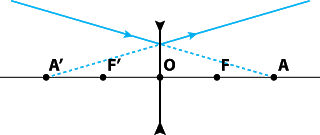
\includegraphics[width=\textwidth]{notaveis_div_4.png}
         \caption{Lente Divergente}
         \label{fig:raios_div_4}
     \end{subfigure}
    \end{figure}
\end{enumerate}

\subsection{Formação de Imagens}
Iremos estudar os casos da formação de imagens por meio de lentes. Ao todo, são 6 casos: 5 para as lentes convergentes e 1 caso geral para a lente divergente.
\begin{enumerate}
    \item \textbf{Quando o objeto está atrás do ponto antiprincipal}
    \begin{figure}[H]
        \centering
        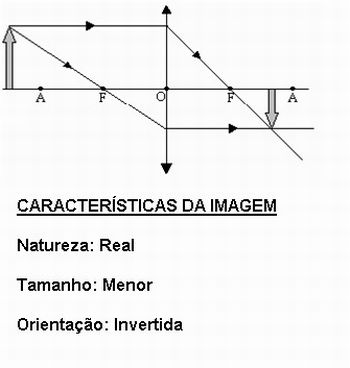
\includegraphics[width=0.4\textwidth]{caso_conv_atras_anti.jpg}
    \end{figure}
    
    \item \textbf{Quando o objeto está no ponto antiprincipal}
    \begin{figure}[H]
        \centering
        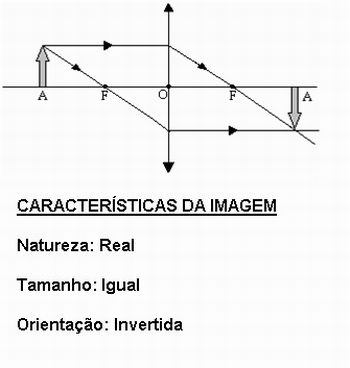
\includegraphics[width=0.4\textwidth]{caso_conv_no_anti.jpg}
    \end{figure}
    
    \item \textbf{Quando o objeto está entre o ponto antiprincipal e o foco}
    \begin{figure}[H]
        \centering
        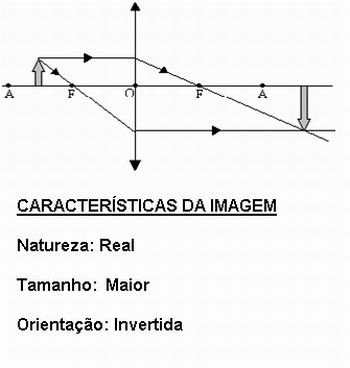
\includegraphics[width=0.4\textwidth]{caso_conv_entre_anti_foco.jpg}
    \end{figure}
    
    \item \textbf{Quando o objeto está no foco}
    \begin{figure}[H]
        \centering
        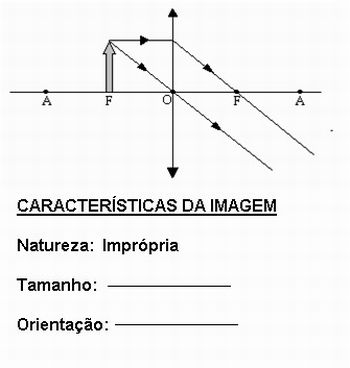
\includegraphics[width=0.4\textwidth]{caso_conv_no_foco.jpg}
    \end{figure}
    
    \item \textbf{Quando o objeto está a frente do foco}
    \begin{figure}[H]
        \centering
        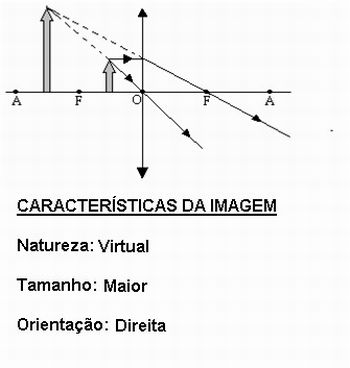
\includegraphics[width=0.4\textwidth]{caso_conv_frente_foco.jpg}
    \end{figure}
    
    \item \textbf{Caso geral - lentes divergente}
    \begin{figure}[H]
        \centering
        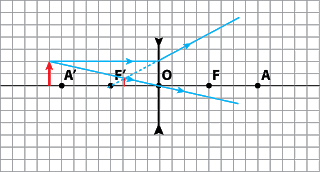
\includegraphics[width=0.4\textwidth]{caso_div.png}
    \end{figure}
    A imagem é Virtual, Direita e Menor.
\end{enumerate}

\subsection{Equações}
As equações para as lentes são as mesmas equações para os espelhos: A equação de Gauss

\begin{equation}
    \frac{1}{f} = \frac{1}{p} + \frac{1}{p'}
\end{equation}

Equação do aumento linear:
\begin{equation}
    A = \frac{i}{o} = -\frac{p'}{p} = \frac{f}{f-p}
\end{equation}
\noindent em que:
\begin{itemize}
    \item 'i' - tamanho da imagem;
    \item 'o' - tamanho do objeto;
    \item 'p' - distância do objeto até a lente;
    \item ' p' ' - distância da imagem até a lente;
    \item 'f' - distância focal
\end{itemize}
\textit{Obs:}
\textbf{Distância focal:}
\begin{itemize}
    \item Lente convergente - 'f' positivo;
    \item Lente divergente - 'f' negativo;
\end{itemize}
\textbf{Distância da imagem até a lente - p'}
\begin{itemize}
    \item Imagem Real - ' p' ' positivo;
    \item Imagem Virtual - ' p' ' negativo;
\end{itemize}
\textbf{Tamanho da imagem - i}
\begin{itemize}
    \item Imagem direita - 'i' positivo;
    \item Imagem Invertida - 'i' negativo
\end{itemize}
\end{document}
